\begin{center}
	\LARGE
	Med hjælpemidler
\end{center}

\begin{opgavetekst}{Opgave 1}
	Grafen for en stykvist lineær funktion $f$ kan ses på Figur \ref{fig:styk}.
	\begin{figure}[H]
		\centering
		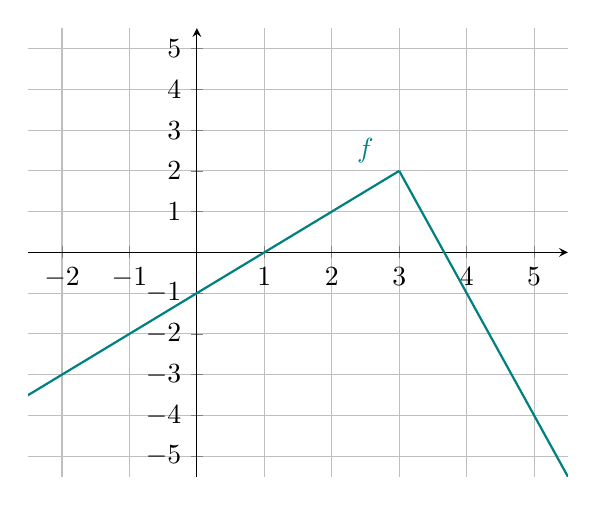
\begin{tikzpicture}
		\begin{axis}[
			axis lines = center,
			xmin = -2.5, xmax = 5.5,
			ymin = -5.5, ymax = 5.5,
			xtick = {-5,-4,...,5,6},
			ytick = {-5,-4,...,5,6},		
			grid = both,
			]
			\addplot[color = teal, thick, domain = -3:3] {x-1};
			\addplot[color = teal, thick, domain = 3:6] {-3*x+11};
			\node[color = teal] at (axis cs: 2.5,2.5) {$f$};
		\end{axis}
		\end{tikzpicture}
		\caption{Graf for funktionen $f$.}
		\label{fig:styk}
	\end{figure}
	\phantom{h}
\end{opgavetekst}
\begin{delopgave}{1}
	Bestem en forskrift for $f$.
\end{delopgave}
\begin{delopgave}{2}
	Bestem skæringspunkterne mellem grafen for $f$ og linjen givet ved
	\begin{align*}
		y = \frac{1}{2}x-4.
	\end{align*}
\end{delopgave}
%
%
%
%
%
\begin{opgavetekst}{Opgave 2}
	En funktion $g$ er givet ved
	\begin{align*}
		g(x) = \frac{x^3}{\sqrt{x^2 + 1}}
	\end{align*}
\end{opgavetekst}
\begin{delopgave}{1}
	Bestem en stamfunktion til $g$, der går gennem punktet $(\sqrt{3},\frac{5}{3})$
\end{delopgave}
%
%
%
%
%
\newpage
\begin{opgavetekst}{Opgave 3}
	En funktion $f$ er givet ved
	\begin{align*}
		f(x) = 0.02x^4 - 0.06x^3 - 0.5x^2 + 0.61x + 3.39.
	\end{align*}
\end{opgavetekst}
\begin{delopgave}{1}
	Tegn grafen for $f$ så $-6 < x < 7$.
\end{delopgave}
\begin{delopgave}{2}
	Bestem koordinatsættene til ekstrema for $f$. 
\end{delopgave}
\begin{delopgave}{3}
	Brug differentialkvotienten for $f$ til at opskrive monotoniforholdene for $f$. 
\end{delopgave}
\begin{delopgave}{4}
	Bestem de værdier for $k$, så linjen $y = k$ har netop 3 røringspunkter med grafen for $f$. 
\end{delopgave}
%
%
%
%
%
\begin{opgavetekst}{Opgave 4}
	Om en funktion $f$ opfyldes det, at 
	\begin{align*}
		f''(x) = x^3+2x-4.
	\end{align*}
	Desuden gælder det, at $f'(4) = 2$ samt $f(3) = -10$.
\end{opgavetekst}
\begin{delopgave}{1}
	Bestem en forskrift for $f$. 
\end{delopgave}
%
%
%
%
%
\begin{opgavetekst}{Opgave 5}
	\begin{center}
		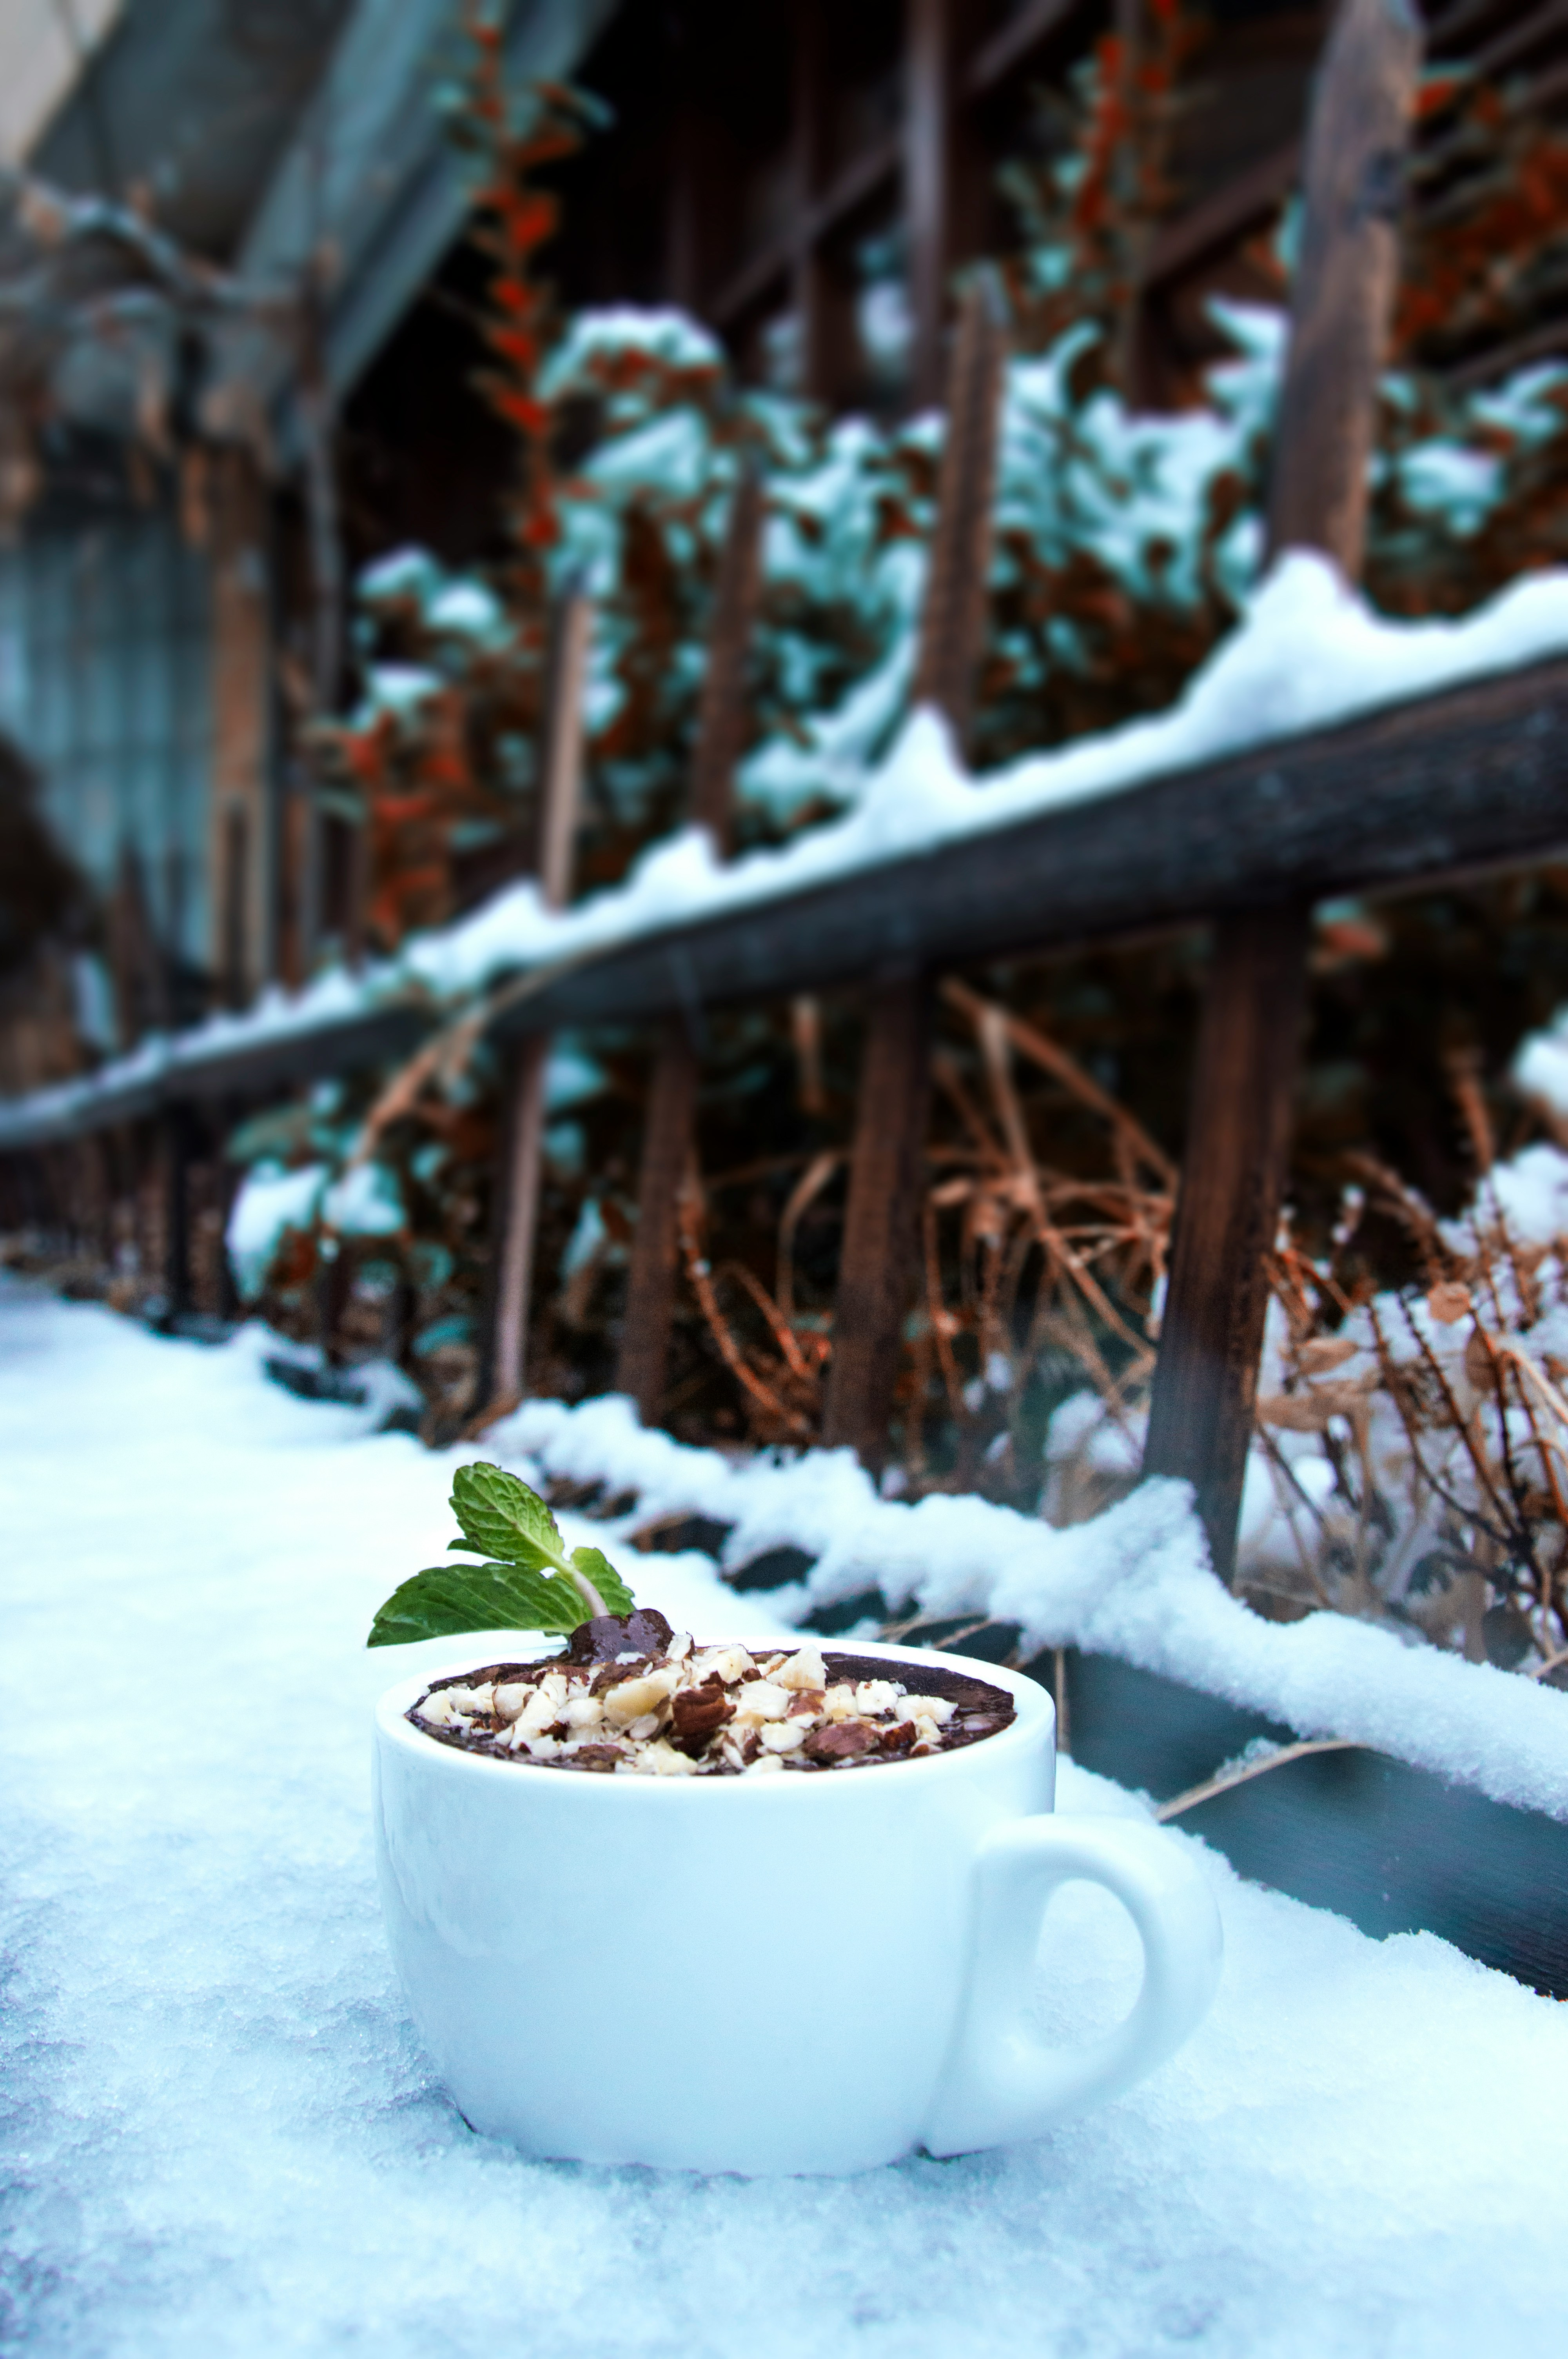
\includegraphics[width=0.35\textwidth]{Billeder/kakao}
	\end{center}
	Det er vinter, og du har serveret dig selv en kop varm kakao. Den står udenfor, og temperaturen af
	kakaoen kan beskrives ved funktionen
	\begin{align*}
		f(t) = 77.8\cdot 0.918^t,
	\end{align*}
	hvor $t$ betegner det forløbne antal minutter og $f$ betegner temperaturen af kakaoen i C$^\circ$.
\end{opgavetekst}
\begin{delopgave}{1}
	Forklar, hvad tallene 77.8 og 0.918 betyder for temperaturen af koppen.
\end{delopgave}
\begin{delopgave}{2}
	Bestem temperaturen af kakaoen efter 20 minutter.
\end{delopgave}
\begin{delopgave}{3}
	Bestem temperaturen af kakaoen, når den aftager med mindre end 1 grad per minut. 
\end{delopgave}
%
%
%
%
%

%
%
%
%
%
\begin{opgavetekst}{Opgave 6}
	Vi skal konstruere en beholder til en pindeis. Den skal være cylindrisk og den skal have et låg som en halvkugle. Vi kan se en illustration af beholderen på Figur \ref{fig:pindeis}.
\begin{figure}[H]
	\centering
	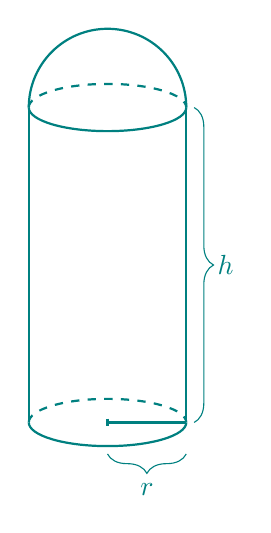
\begin{tikzpicture}  
		%Sides
		\draw[color = teal, thick] (0,0) -- (0,4);
		\draw[color = teal, thick] (2,0) -- (2,4);
		%Buttom and top
		\draw[color = teal, thick] (0,0) arc [start angle = 180, end angle = 360,
		 x radius = 1cm, y radius = 0.3cm];
		\draw[color = teal, thick, dashed] (0,0) arc [start angle = 180, end angle = 0,
		 x radius = 1cm, y radius = 0.3cm]; 
		 \draw[color = teal, thick] (0,4) arc [start angle = 180, end angle = 360,
		 x radius = 1cm, y radius = 0.3cm];
		\draw[color = teal, thick, dashed] (0,4) arc [start angle = 180, end angle = 0,
		 x radius = 1cm, y radius = 0.3cm]; 
		 %Half-ball
		 \draw[color = teal, thick] (0,4) arc [start angle = 180, end angle = 0, radius = 1cm];
		 %Braces
		 \draw[decorate,decoration = {brace,amplitude = 7pt, mirror},color = teal] (2.1,0) -- (2.1,4);
		 \node[color = teal] at (2.5,2) {$h$};
		 \draw[decorate,decoration = {brace,amplitude = 7pt, mirror},color = teal] (1,-0.4) -- (2,-0.4);
		 \node[color = teal] at (1.5,-0.85) {$r$};
		 \draw[color = teal, thick] (2,0) -- (1,0);
		 \draw[color = teal, thick] (1,0.05) -- (1,-0.05);
	\end{tikzpicture}
	\caption{Beholder til is.}
	\label{fig:pindeis}
\end{figure}
Beholderen skal have en bund, en side og låget, der alle er i samme materiale. Den skal indeholde 150 mL is, og rumfanget skal være så småt som muligt. 
\end{opgavetekst}
\begin{delopgave}{1}
	Bestem et udtryk for rumfanget og sæt dette lig 150.
\end{delopgave}	
\begin{delopgave}{2}
	Bestem et udtryk for overfladearealet og brug dit svar fra a) til at bestemme dimensionerne for beholderen, der gør
	overfladearealet så småt som muligt. 
\end{delopgave}
